\chapter{Конструкторская часть}

\section{Концептуальный дизайн}
Для создания функциональной модели портала, отражающей его основные функции и потоки информации наиболее наглядно использовать нотацию IDEF0. На рисунке \ref{fig:idef0-0} приведена концептуальная модель системы. На рисунке \ref{fig:idef0-1} представлена детализированная концептуальная модель системы в нотации IDEF0.

\begin{figure}[h!]
	\begin{center}
		{\includegraphics[scale = 0.5, angle=0]{../img/idef0/idef0-0.png}}
		\caption{Концептуальная модель системы в нотации IDEF0}
		\label{fig:idef0-0}
	\end{center}
\end{figure}


\begin{figure}[h!]
	\begin{center}
		{\includegraphics[scale = 0.4, angle=90]{../img/idef0/idef0-1.png}}
		\caption{Детализированная концептуальная модель системы в нотации IDEF0}
		\label{fig:idef0-1}
	\end{center}
\end{figure}


\clearpage
\section{Сценарии функционирования системы}

\textbf{Регистрация пользователя}
\begin{enumerate}
	\item Пользователь нажимает на кнопку <<Зарегистрироваться>> в интерфейсе.
	\item Пользователь перенаправляется на страницу, которая содержит поля для заполнения его данных.
	\item Пользователь вводит данные в форму и для завершения регистрации нажимает на кнопку <<Зарегистрироваться>>, тем самым подтверждая верность своих данных, а также согласие на их обработку и хранение.
	\item Если пользователь с введенным для регистрации логином, почтой или номером телефона уже существует, то клиент получает сообщение об ошибке. При успешной регистрации клиент попадает на страниицу со списком полетов.
\end{enumerate}

\textbf{Авторизация клиента}
\begin{enumerate}
	\item Пользователь нажимает на кнопку <<Авторизоваться>> в интерфейсе.
	\item Пользователь перенаправляется на страницу авторизации, которая содержит поля для заполнения логина и пароля.
	\item Пользователь завершает работу с формой авторизации нажатием кнопки <<Войти>>.
	\item При обнаружении ошибки в данных, пользователь получает сообщение об ошибке; при совпадении данных с записью в базе данных аккаунтов пользователь получает доступ к системе и перенаправляется на страниицу со списком полетов.
\end{enumerate}

\textbf{Покупка билета}
\begin{enumerate}
	\item Пользователь на главной странице видит таблицу со списком список полетов. При желании он может отфильтровать и отсортировать их по каждому полю.
	\item Пользователь нажимает на кнопку <<Купить билет>> у выбранного рейса.
  \item Пользователь выбирает, что делать с бонусами (списать или копить) и нажимает кнопку <<Забронировать>>.
  \item В появившемся модальном окно подтверждения с подробной информацией о выбранном рейсе пользователь нажимает на кнопку <<Подтвердить>>.
	\item Пользователь видит модальное окно с информацией об успешности совершенной покупки и нажимает кнопку <<Окей>>.
\end{enumerate}

\textbf{Возврат купленного билета}
\begin{enumerate}
	\item Для просмотра купленных билетов пользователь переходит на страницу <<Билеты>>, нажимая соответсвующую кнопку в выезжающем боковом меню.
	\item Пользователь попадает на страницу, на которой видит все свои купленные и сданные билеты.
	\item У каждого купленного билета есть кнопка <<Сдать билет>>, на которую нажимает пользователь.
	\item В появившемся модальном окно подтверждения с подробной информацией о выбранном билете пользователь нажимает на кнопку <<Подтвердить>>.
  \item Пользователь видит измененный статус билета на <<Билет сдан>> и обновленный баланс бонусного счета.
\end{enumerate}


\section{Диаграммы прецедентов}
В системе выделены 3 роли: Неавторизованный пользователь, Авторизованный пользователь, Администратор. На рисунках \ref{fig:use-case-non-auth}-\ref{fig:use-case-admin} представлены диаграммы прецедентов для каждой из ролей.

\begin{figure}[H]
	\begin{center}
		{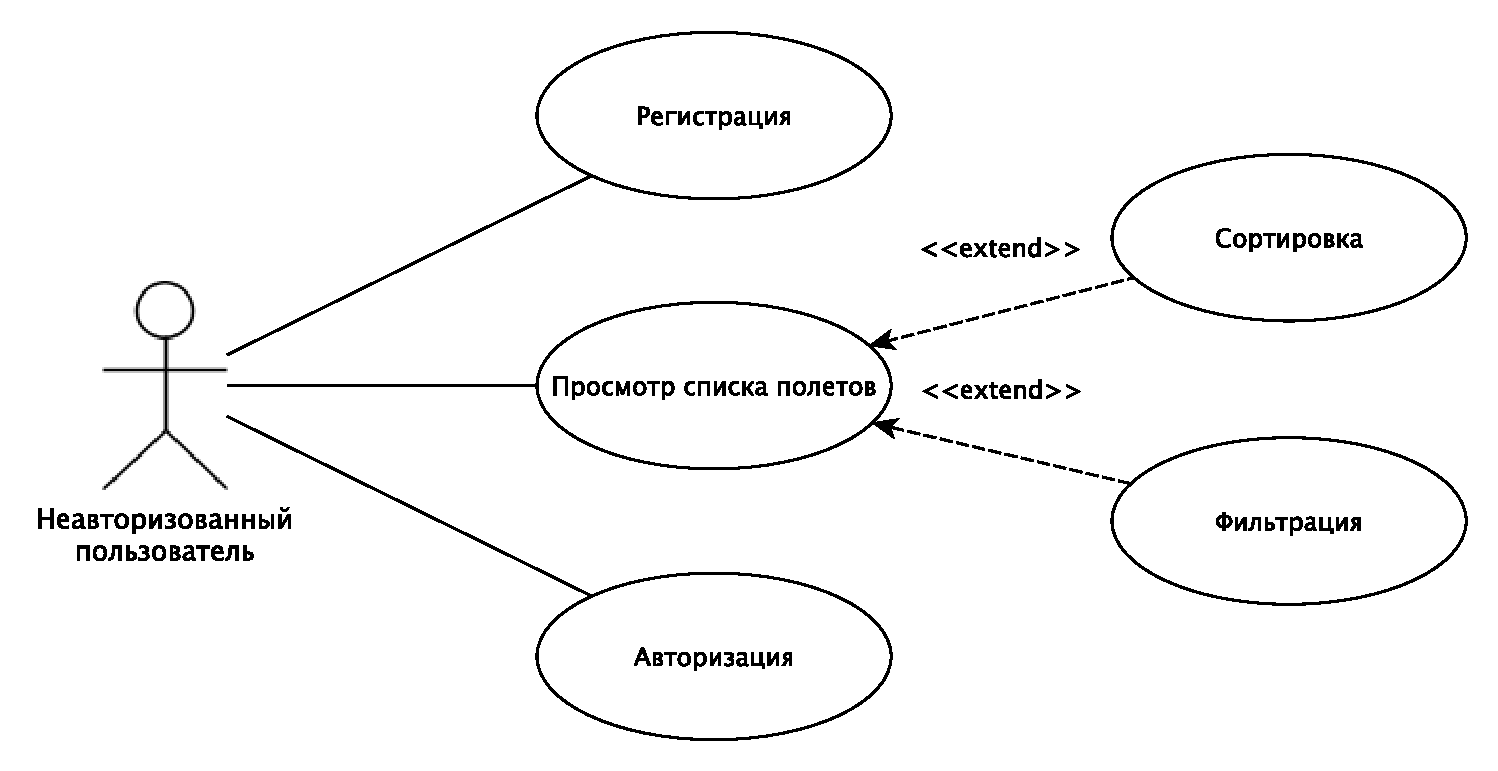
\includegraphics[scale = 0.5]{../img/use-case/non-auth-user.pdf}}
		\caption{Диаграмма прецедентов с точки зрения Неавторизованного пользователя}
		\label{fig:use-case-non-auth}
	\end{center}
\end{figure}

\begin{figure}[H]
	\begin{center}
		{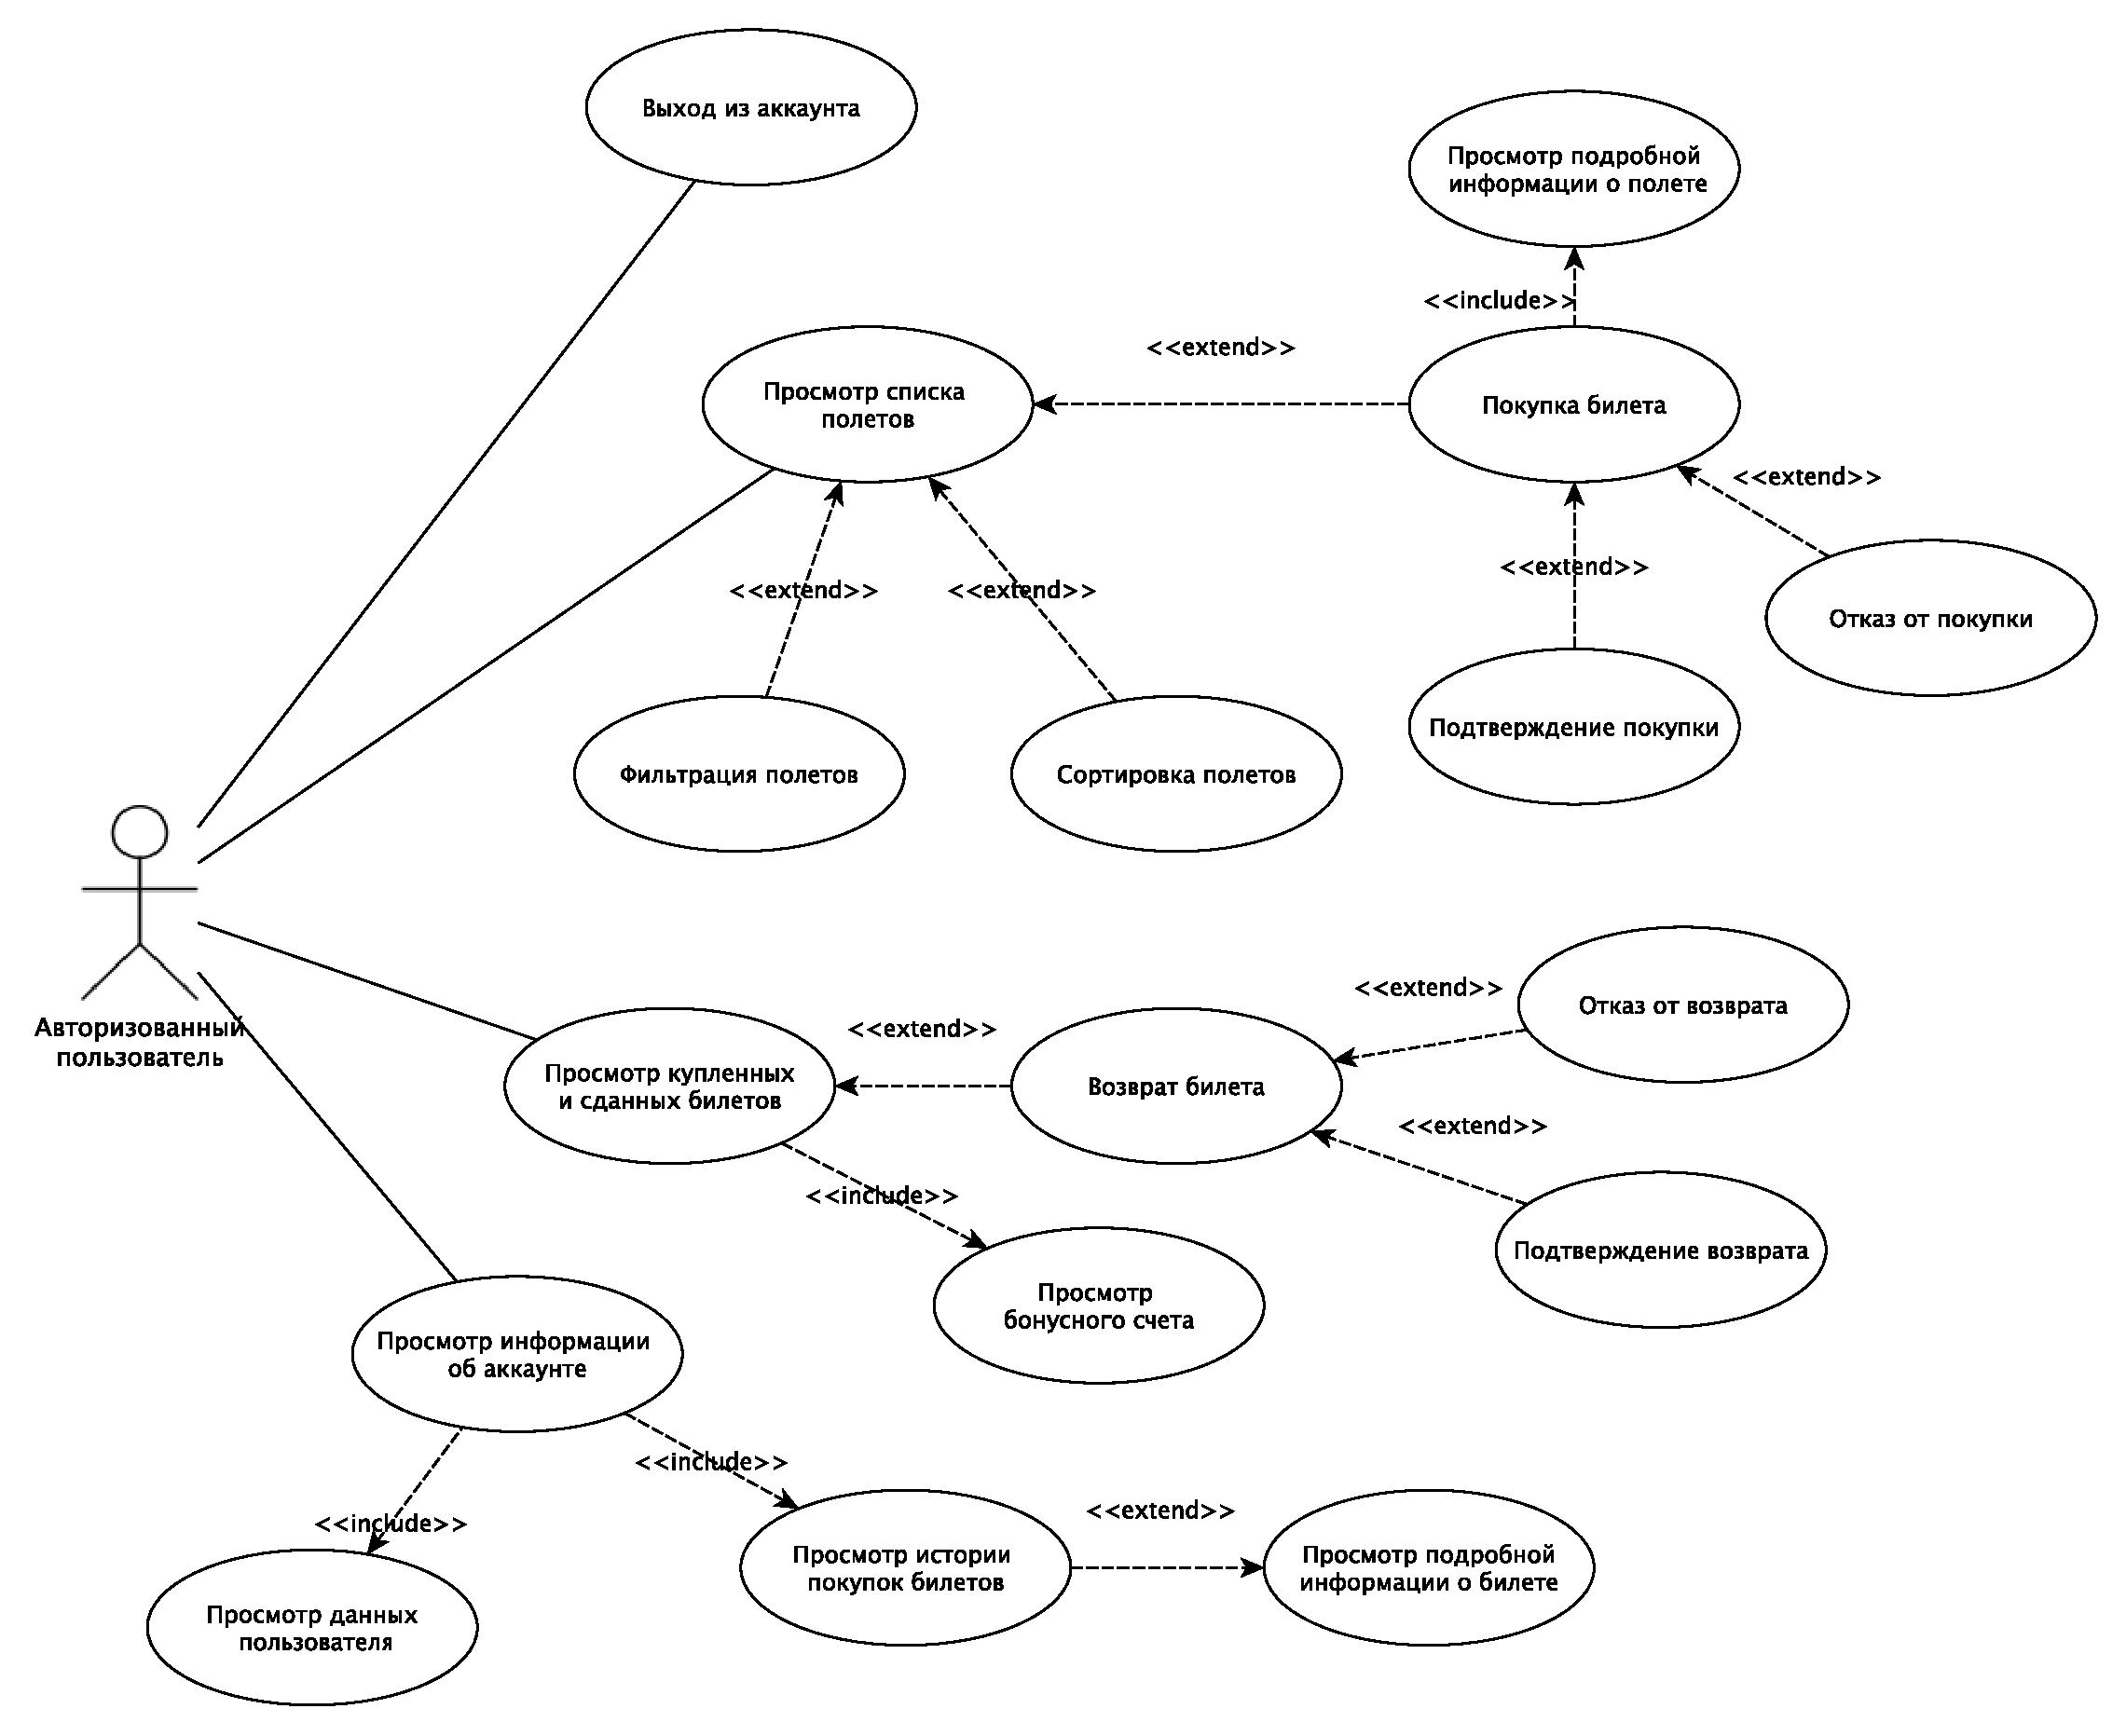
\includegraphics[scale = 0.4]{../img/use-case/auth-user.pdf}}
		\caption{Диаграмма прецедентов с точки зрения Авторизованного пользователя}
		\label{fig:use-case-auth}
	\end{center}
\end{figure}

\begin{figure}[H]
	\begin{center}
		{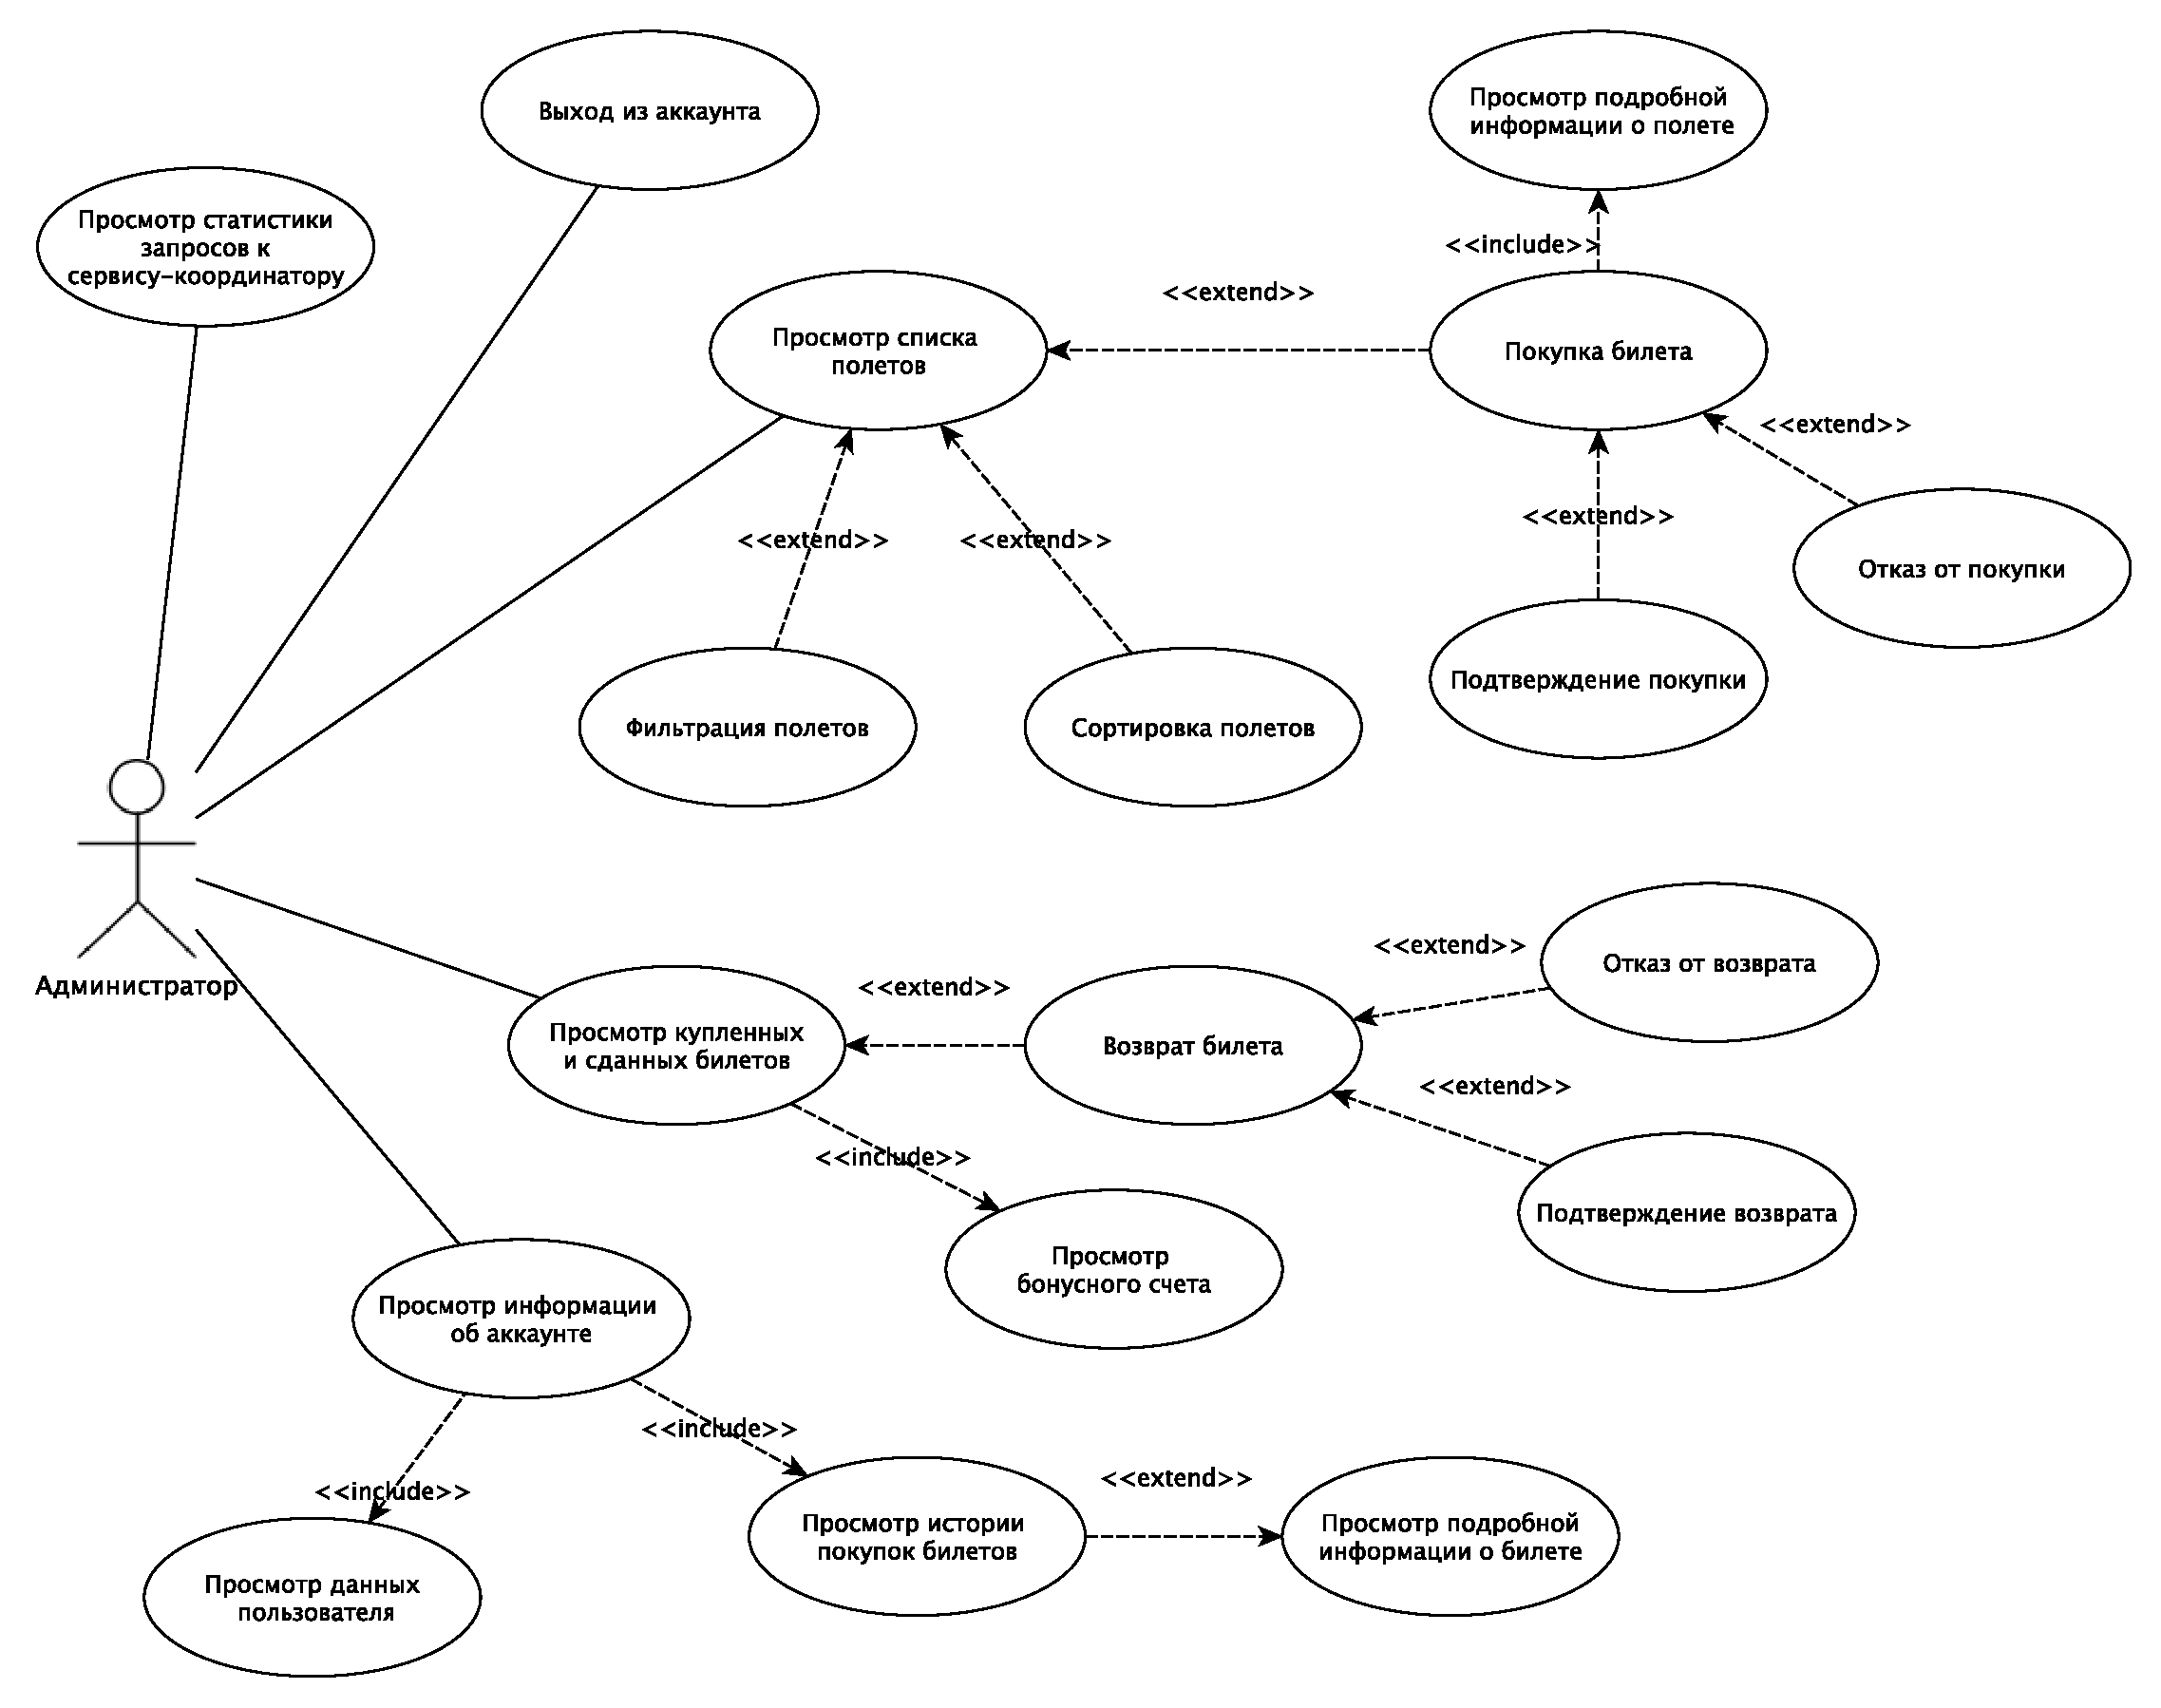
\includegraphics[scale = 0.45]{../img/use-case/admin.pdf}}
		\caption{Диаграмма прецедентов с точки зрения Администратора}
		\label{fig:use-case-admin}
	\end{center}
\end{figure}
